\documentclass[french,frtypo,twoside,actes,a4paper]{article}
\usepackage[latin1]{inputenc}
\usepackage[T1]{fontenc}
\usepackage{actes,hyperref,graphicx}
%% Title page...
\title{ReML : une biblioth�que OCaml pour la combinatoire}
\author{R�my El Siba�e$^1$
  \& Jean-Christophe Filli�tre$^{2,1}$}
%% Headers for other pages...
\titlehead{ReML : une biblioth�que OCaml pour la combinatoire} % for odd pages
\authorhead{R.~El Sibaie \& J.-C. Filli�tre}     % for even pages
\affiliation{\begin{tabular}{rr}        % for institute(s)
    \\ 1:  LRI, Universit� Paris Sud,
    \\     91405 Orsay CEDEX, France
    \\ 2:  CNRS,
    \\     {\tt remy.el-sibaie@u-psud.fr}
    \\     {\tt jean-christophe.filliatre@lri.fr}
  \end{tabular}}

\newcommand{\reml}{ReML}

\begin{document}
\setcounter{page}{1}
\maketitle

\begin{abstract}
  Cet article pr�sente \reml, une biblioth�que OCaml pour la
  combinatoire\footnote{Il s'agit d'un travail r�alis� par le premier
    auteur pendant un stage de L3 au LRI, d'avril � juin 2012, sous la
    direction du second auteur.}.
\end{abstract}

\section{Introduction}

\begin{center}
  \includegraphics{caml_problem.mps}
\end{center}
\begin{center}
  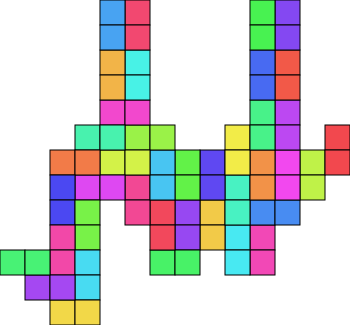
\includegraphics{caml_solution.mps}
\end{center}

caml
46976 solutions
(ZDD 0.11s, DLX 0.09s)

\begin{center}
  \includegraphics{caml2_problem.mps}
\end{center}

caml2
32,420,116,341,024,288 solutions
(ZDD 39.7s, 1.4 Go de RAM)


\cite{taocp4a}

\cite{knuth00:dlx}

\cite{ZDD}

Mlpost~\cite{mlpost09jfla}

La biblioth�que \reml\ est un logiciel libre, distribu� sous licence
LGPL � l'adresse \url{http://www.lri.fr/~filliatr/reml/}.

\section{Architecture}

La biblioth�que \reml\ fournit :
\begin{itemize}
\item l'algorithme \emph{Dancing Links} de Knuth
\item la structure de ZDD
\item
\item 
\end{itemize}

\section{R�alisation} % = d�tails techniques


\section{Conclusion et perspectives}


% And do NOT FORGET to include your bibliography for submission
\bibliographystyle{plain}
\bibliography{abbrevs,demons,demons2,demons3,team,crossrefs,crossrefs2}

\vfill
\pagebreak
\thispagestyle{colloquetitle}
\cleardoublepage
\end{document}

%%% Local Variables:
%%% mode: latex
%%% ispell-local-dictionary: "francais"
%%% TeX-master: t
%%% End:
